\documentclass[xcolor=dvipsnames]{beamer} 
\setbeamertemplate{blocks}[rounded][shadow=false]

%\usetheme{Boadilla}
%\usetheme{Frankfurt}
%\usetheme{}
%\usetheme{}
%\usetheme{}
%\usetheme{}
%\usetheme{}
%\usetheme{}
\usetheme{Madrid}

\setbeamertemplate{items}[square]



\usepackage{float}
\usepackage[brazil]{babel}
\usepackage[utf8]{inputenc}

\usepackage{graphicx}
\usepackage{url}
\usepackage{float}     % para forçar a localizaçao das figuras (usando H no posicionamento, =Here)
\usepackage[]{subfigure}

\usepackage{scalefnt}
\usepackage{ragged2e}
\usepackage{etoolbox}


\newcommand{\aspas}[1]{``#1''}

\let\olditem=\item% 
\renewcommand{\item}{\olditem \justifying}%

%\usetheme{Antibes}
%\usetheme{Berlin}

\title[HTA]{HTA - \textit{Hierarchical Task Analysis}}
\subtitle{Seminário de Interface Humano-Computador -- \\Bacharelado em Ciência da Computação}
\author[César, Ramos, Guimarães]
{João Paulo Fernandes Cerqueira César, Natanael Ramos, Rodolfo Labiapari Mansur Guimarães}
\institute[IFMG]{Instituto Federal de Educação, Ciência e Tecnologia de Minas Gerais (IFMG) \\ - \textit{campus} Formiga}
\date[\today]{\today}

\begin{document}
\frame{\titlepage}

\AtBeginSection[] 
{
	\begin{frame}
	\frametitle{Sumário}
	\tableofcontents[currentsection]
	\end{frame}
}



\section{Introdução}

\begin{frame}{História}

  \begin{itemize}
  
      \item Metodologia desenvolvida na década de 60 (HOLLNAGEL, 2003);
      
      
      \begin{itemize}
      
		\item Inicialmente foi utilizado em indústrias de aço e petroquímicas.
        
	  \end{itemize}
      
      \bigskip
      
      
		%A Psicologia Funcional , como o próprio nome indica, interessa-se pelo funcionamento da mente.
		%Os psicólogos funcionalistas estudavam a mente.
      
	  \item Adotada pela ciência cognitiva;
      
      \bigskip
      
	  \item Se baseia em psicologia funcional e não comportamental como era comum na época de sua criação (ANNETT; DUNCAN, 1967).
	  
	  \bigskip
	  
	  \item Relacionar \textbf{o que} as pessoas fazem, \textbf{por que} o fazem e as \textbf{consequências} caso não o façam corretamente (BARBOSA; SILVA, 2010).
      
  \end{itemize}
  
\end{frame}



\begin{frame}{Princípios (HOLLNAGEL, 2003)}

  \begin{itemize}
  
  	\item Realizar uma análise hierárquica de tarefas complexas e não repetitivas (BARBOSA; SILVA, 2010);
    
    \bigskip
    
	\item Construído em cima de tarefas e objetivos;
    
    \bigskip
    
    \item Baseado no princípio onde objetivos são utilizados para mensurar o grau de sucesso ou fracasso de um projeto;
    
    \bigskip
    
    \item Objetivos podem ser:
    
    	\begin{itemize}
        
        	\item \textbf{Ativos:} os quais estão sendo atualmente sendo trabalhados;
            
            \bigskip
            
            \item \textbf{Latentes:} os quais serão trabalhados quando determinadas condições ocorrerem.
            
    	\end{itemize}
        
  \end{itemize}
  
\end{frame}




\section{Conceitos}


\begin{frame}{Elementos do HTA  (BARBOSA; SILVA, 2010)}

	\begin{itemize}
    
    	\item \textbf{Tarefas:} qualquer parte do trabalho que precisa ser realizado.
        
        \bigskip
        
		\item \textbf{Objetivos:} estado específico, alvo, tratado como um estado final.
        
        \bigskip
        
        \item \textbf{Plano:} define subobjetivos necessários para alcançar um outro objetivo maior.
        
        \bigskip
        
        \item \textbf{Operações:} unidade fundamental da HTA, especifica como cada subobjetivo é alcançado.
        
    \end{itemize}
    
      	\begin{figure}[H]
    	\centering
        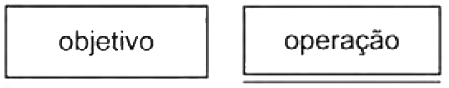
\includegraphics[width=0.75\linewidth]{img/elementos.png}
        \caption{Elementos de um diagrama HTA. Fonte: (BARBOSA; SILVA, 2010).}

    \end{figure}
    
\end{frame}



\begin{frame}{Decomposição e Redescrição  (HOLLNAGEL, 2003)}

	\begin{itemize}
    
    	\item Objetivos são geralmente complexos;
        
        
        \begin{itemize}
        
			\item Possuem múltiplos eventos e múltiplas variáveis.
            
		\end{itemize}
        
        \bigskip
        
    	\item O processo de especialização de componentes de objetivos é chamado de \textbf{decomposição} ou \textbf{redescrição};
        
        
    \end{itemize}
    
\end{frame}


\begin{frame}{Decomposição e Redescrição  (HOLLNAGEL, 2003)}

	\begin{itemize}
    
    	
    	\item HTA define dois tipos de decomposição que, respectivamente, consistem em identificar:
        
        
		\begin{itemize}
        
			\item Estados de objetivo definidos por múltiplos critérios;
            
            \bigskip
            
			\item Subobjetivos em qualquer rota que possa ser seguida para alcançar o objetivo principal.
		\end{itemize}
        
        \bigskip
        
		\item O processo de decomposição de objetivos em subobjetivos revela uma estrutura aninhada hierárquica;
        
        \bigskip
        
		\item Auxilia a busca por erros em um sistema.
        
    \end{itemize}
    
\end{frame}


\begin{frame}{Operações: \textit{Input}, \textit{Action} e \textit{Feedback}  (HOLLNAGEL, 2003)}

	\begin{itemize}
    
		\item Uma operação é definida por um objetivo:
        
        \bigskip
        
		\begin{itemize}
        
			\item \textbf{\textit{Input:}} circunstâncias em que o objetivo é ativado;
            
            \bigskip
            
			\item \textbf{\textit{Action:}} atividades que contribuem para a realização do objetivo;
            
            \bigskip
            
			\item \textbf{\textit{Feedback:}} condições que indicam a realização do objetivo.
            
		\end{itemize}
        
        
	\end{itemize}
    
\end{frame}


\begin{frame}{Operações: \textit{Input}, \textit{Action} e \textit{Feedback}}

	\begin{itemize}

        
		\item Operações devem ser divididas em suboperações:
        
        \bigskip
        
		\begin{itemize}
        
			\item Suboperações são arranjadas de formas a estarem em ordens elevadas a suas respectivas operações (subordinadas);
            
            \bigskip
            
			\item As suboperações subordinadas constituindo uma operação devem ser mutualmente exclusivas e exaustivas:
            
            \bigskip
            
			\begin{itemize}
            
				\item Devem definir completamente o objetivo a que estão subordinados;
                
                \bigskip
                
				\item Sem que haja sobreposições entre os subobjetivos.
                
			\end{itemize}
            
		\end{itemize}      
		
	\end{itemize}
    
\end{frame}



\begin{frame}{Operações: \textit{Input}, \textit{Action} e \textit{Feedback}  (HOLLNAGEL, 2003)}

	\begin{block}{Exemplo (BARBOSA; SILVA, 2010)}
        
        \bigskip
        
		\texttt{\textless inputs, ações, feedback\textgreater:}
        
        \bigskip
        
        \begin{itemize}

			\item \textbf{inputs:} \texttt{[data, local, participantes]},
            \item \textbf{ações:} \texttt{[convidar os participantes]}, 
            \item \textbf{\textit{feedback:}} \texttt{[presença dos participantes confirmada]}.

		\end{itemize}
        
		
	\end{block}
    
\end{frame}


\begin{frame}{Planos}

  	\begin{figure}[H]

    	\centering
        \label{fig:taskarchitect}
        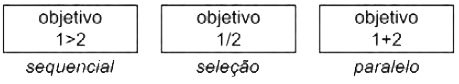
\includegraphics[width=0.75\linewidth]{img/planos.png}
        \caption{Tipos de Planos em um diagrama HTA. Fonte: (BARBOSA; SILVA, 2010).}

    \end{figure}

	\begin{itemize}
    
		\item Consiste no conjunto de regras que definem a ordem em que as operações e suboperações devem ser executadas;
        
        \bigskip
        
        
		\item \textbf{Sequência fixa ou procedimento de rotina:} ``Faça isso, isso e isso'';
        
        \bigskip
        
		\item \textbf{Regra seletiva ou decisão:} ``Se $x$ acontece, faça isso, caso $y$ aconteça, faça outro''.
            
	\end{itemize}
    
\end{frame}



\begin{frame}{Planos (HOLLNAGEL, 2003)}

	\begin{itemize}
    
		\item \textbf{Compartilhamento de tempo ou dupla tarefa:}
        
        	\bigskip
            
			\begin{itemize}
            
				\item Duas atividades devem ser executadas em paralelo;
                
                \bigskip
                
				\item O objetivo superior não pode ser realizado enquanto dois ou mais subobjetivos não forem executados ao mesmo tempo.
                
                \bigskip
                
				\item Quando um objetivo se torna ativo, todos os objetivos subordinados devem ser ativos também.
                
			\end{itemize}
            
	\end{itemize}
    
\end{frame}



\begin{frame}{Regras de Parada (HOLLNAGEL, 2003)}

	\begin{block}{Quando parar a decomposição?}
    
		Quando tiver toda a informação necessária para o propósito da análise;

	\end{block}
    
    \pause    
    
    \begin{block}{Quando parar a decomposição?}
    
        
		Metodologia $p \times c$:
            
			\begin{itemize}
            
				\item \aspas{Parar quando o produto da probabilidade de falha ($p$) e custo de falha ($c$) é aceitável};
                
                \bigskip
                
				\item Foca o analista aos aspectos da tarefa que são críticos ao sucesso do sistema como um todo.
                
			\end{itemize}

	\end{block}
    
\end{frame}



\begin{frame}{Regras de Parada (HOLLNAGEL, 2003)}

	\begin{block}{Quando parar a decomposição?}
    
		Em propósito de \textit{design}, pode se decompor até a especificação de equipamentos ou até operações que necessitem de comunicação e colaboração entre os indivíduos envolvidos.

	\end{block}

\end{frame}



\section{Metodologia}


\begin{frame}{Metodologia}
    
	% Oliveira
	% ver página 201 do PDF
        
	Diaper e Stanton (2003) definem os seguintes passos para construir uma HTA:
    
    \bigskip
        
    \begin{enumerate}

		\item \textbf{Decidir os objetivos da análise:} modificar/criar o sistema existente e desenvolver treinamentos;

		\bigskip            

		\item \textbf{Obter consenso entre as partes interessadas na definição dos objetivos da tarefa e medidas de sucesso:} definir frequência de erros e a forma que são aferidos. ``Qual a consequência na falha de concluir o objetivo?'';

		\bigskip            

		\item \textbf{Identificar as fontes de informações das tarefas e selecionar as formas de aquisição de dados:} escolher melhores formas de coleta e como serão realizadas;

	\end{enumerate}
        
\end{frame}



\begin{frame}{Metodologia}
                
	\begin{enumerate}

		\setcounter{enumi}{3}

		\item \textbf{Coletar dados e esboçar uma tabela ou diagrama de decomposição:} realizar a construção de um diagrama para facilitar a visão como um todo;

		\bigskip

		\item \textbf{Verificar a validade da decomposição:} junto com os \textit{stakeholders};

		\bigskip

		\item \textbf{Identificar operações significativas:} nível de aprofundamento aceitável;

		\bigskip            

		\item \textbf{Gerar e testar hipóteses relacionadas aos fatores que afetam o aprendizado e o desempenho:} verificar o desempenho baseado em habilidades, regras ou em conhecimento entre outras técnicas.

	\end{enumerate}
        
\end{frame}




\section{Exemplos}



\begin{frame}{Exemplo de Hierarquia}

	\begin{figure}[H]
    
		\centering
		\caption{Diagrama HTA, para o objetivo de cadastrar um projeto final em um sistema acadêmico (BARBOSA; SILVA, 2010).}
		\label{fig:HTAExHi}
		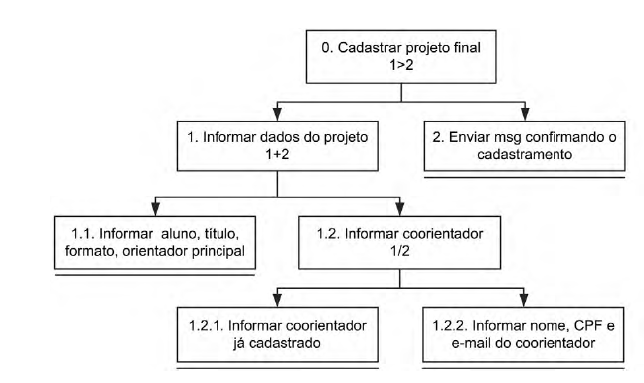
\includegraphics[width=0.8\linewidth]{img/hierarquia}
        
	\end{figure}
    
\end{frame}



\begin{frame}{Exemplo Tabular}

	\begin{figure}[H]
    
		\centering
		\caption{Exemplo de representação das tarefas da HTA em tabela (BARBOSA; SILVA, 2010)}
		\label{fig:tabular}
		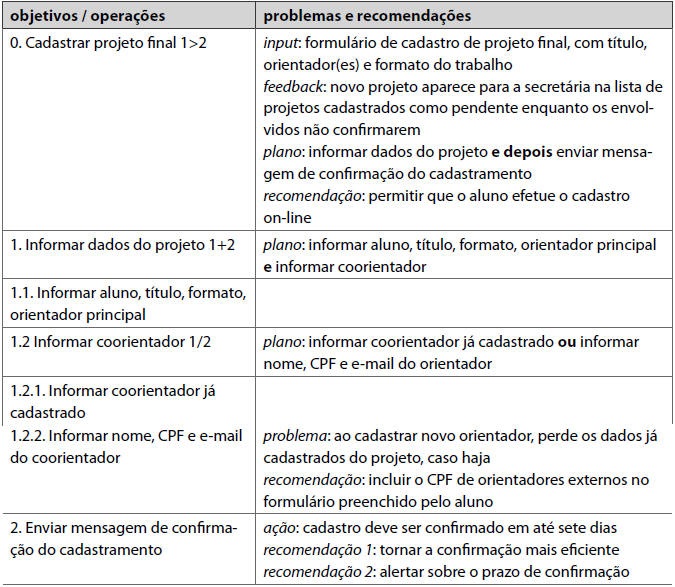
\includegraphics[width=0.6\linewidth]{img/tabular}
        
	\end{figure}

\end{frame}



\section{Ferramentas Computacionais}



\begin{frame}{Ferramentas Computacionais - \href{http://taskarchitect.com/products.html}{Task Architect}}
  
	\begin{figure}[H]
    
    	\centering
        \label{fig:taskarchitect}
        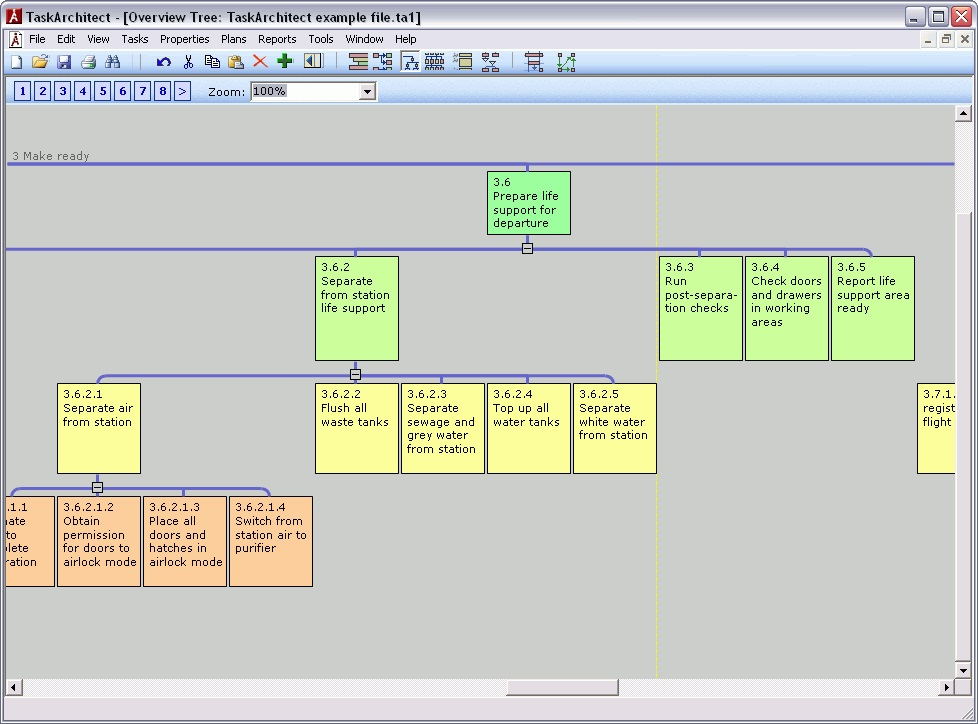
\includegraphics[width=0.7\linewidth]{img/taskarchitect.jpg}
        \caption{Software Task Architect \footnote{\url{http://taskarchitect.com/Pix/Overview-Levels-l.gif}}.}
        
	\end{figure}
    
\end{frame}

%Ferramentas para construção de WBS (\textit{Work Breakdown Structure}), muito similar à HTA:

\begin{frame}{Ferramentas Computacionais - \href{http://www.wbstool.com/}{WBS Tool}}

	\begin{figure}[H]
    
     	\centering
        \label{fig:taskarchitect}
        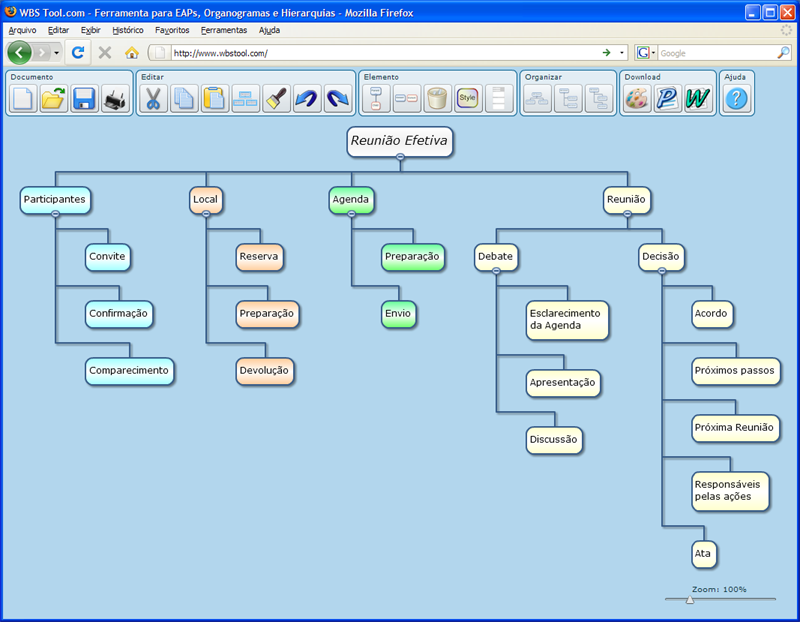
\includegraphics[width=0.68\linewidth]{img/WBSToolScreenShot.png}
        \caption{Software WBS Tool \footnote{\url{http://www.wbstool.com/WBSToolScreenShot.png}}.}
        
	\end{figure}
    
\end{frame}



\begin{frame}{Ferramentas Computacionais - \href{http://www.matchware.com/en/products/mindview/mindview2_be/wbs.htm}{MindView}}

	\begin{figure}[H]
    
     	\centering
        \label{fig:taskarchitect}
        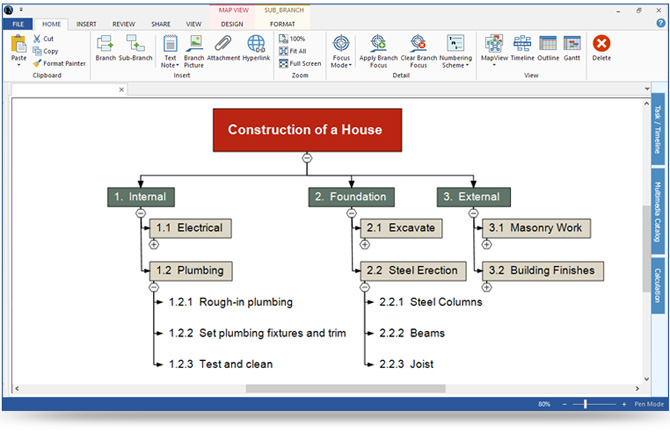
\includegraphics[width=0.8\linewidth]{img/mindview.jpg}
        \caption{Software MindView \footnote{\url{http://www.matchware.com/img/Work-Breakdown-Structure-at-glance.jpg}}.}
        
	\end{figure}
    
\end{frame}



\begin{frame}{Ferramentas Computacionais - \href{http://www.criticaltools.com/WBSChartPro.html}{WBS Chart Pro}}

	\begin{figure}[H]
    
     	\centering
        \label{fig:taskarchitect}
        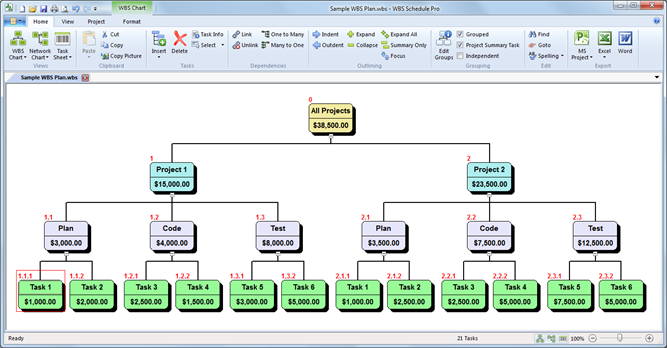
\includegraphics[width=0.9\linewidth]{img/wbs_schedule.png}
        \caption{Software WBS Chart Pro \footnote{\url{http://www.criticaltools.com/images/WBS\%20Main2.png}}.}
        
	\end{figure}
    
\end{frame}



\begin{frame}{Ferramentas Computacionais - \href{http://www.wbstool8.com/en/Start.aspx}{WBStool8}}

	\begin{figure}[H]
    
     	\centering
        \label{fig:taskarchitect}
        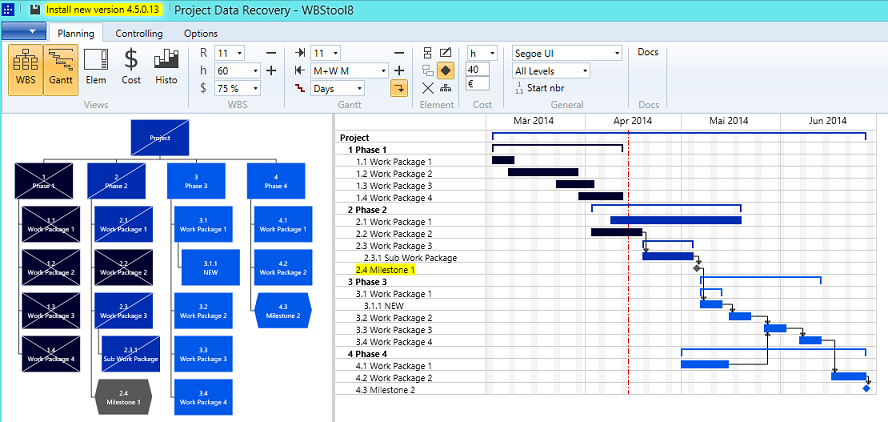
\includegraphics[width=0.9\linewidth]{img/wbstool8.png}
        \caption{Software WBStool8 \footnote{\url{http://www.office-loesung.de/files/wbstool8.png}}.}
        
	\end{figure}
    
\end{frame}



\section{Bibliografia}

\begin{frame}{Bibliografia}
	

\begin{thebibliography}{}
	
	\bibitem{BARBOSA2010}BARBOSA, Simone D. J.; SILVA, Bruno Santana da. Interação humano-computador. Rio de Janeiro: Elsevier, c2010. 384 p. ISBN 9788535234183

	\bibitem{Diaper2003}DIAPER, Dan; STANTON, Neville (Ed.). The handbook of task analysis for human-computer interaction. CRC Press, 2003.

	\bibitem{Hollnagel2003}HOLLNAGEL, Erik (Ed.). Handbook of cognitive task design. CRC Press, 2003.	
		
	\end{thebibliography}

\end{frame}

\end{document}
